\chapter{Fravælgelse af gestik-par}
\label{app:TestresultaterFravaelgelse}
%
I følgende kapitel vil fravælgelsen af diverse gestik-par dokumenteres i forhold til testpersonernes respons, først i forhold til pause og start, dernæst i forhold til at skifte musiknummer og slutteligt i forhold til justering af lydstyrken. 
%
\section{Fravælgelse af gestik-par til pause og start}
\label{app:TestresultaterPauseDaarlig} 
%
I følgende afsnit analyseres det, hvilke af de syv semaforiske gestik-par testpersonerne fravælger samt hvorfor testpersonerne netop fravælger disse gestik-par. På baggrund af analysen, bør det være muligt at udpege, hvilke semaforiske gestikker, der i hvert fald ikke skal knyttes til hverken pause eller start. Analysen bygger på testpersonerne respons til spørgsmålet: \textit{Hvilken gestik kan du mindst lide? og hvorfor?}, hvor testpersonernes samlede data er vedlagt i \autoref{app:NoterValgAfGestikker}.
%
\begin{figure}[H]
	\centering
	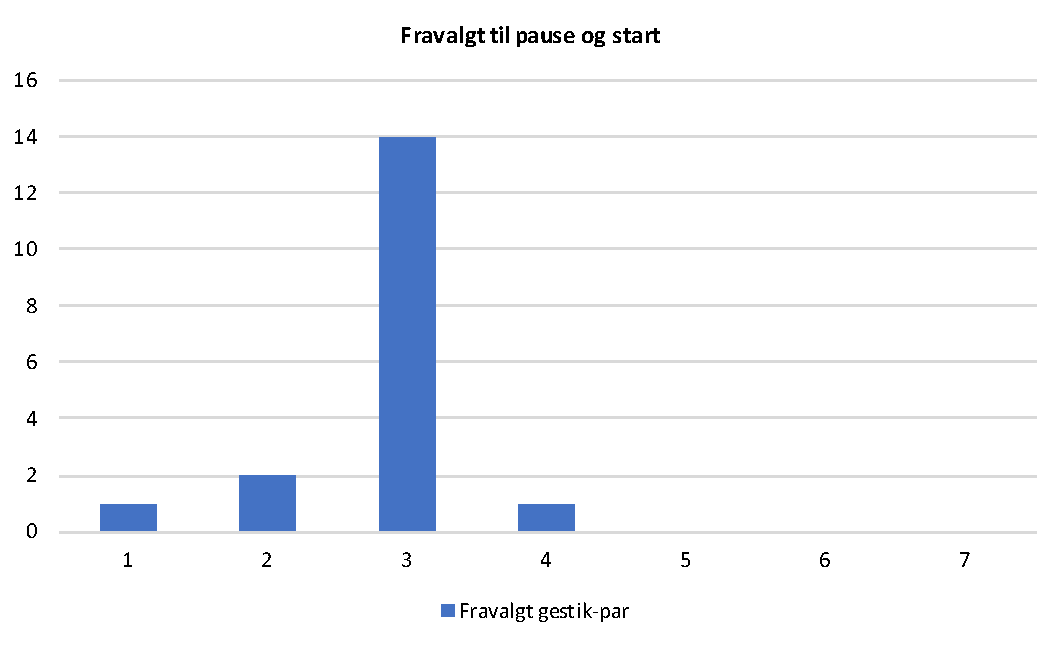
\includegraphics[resolution=300,width=0.9\textwidth]{Test1/DatabehandlingGrafer/FravalgtPause}
	\caption{Søjlediagram over hvilke gestik-par testpersonerne fravælger i forbindelse med pause og start.}
	\label{fig:DaarligstGestikPause}
\end{figure}
\noindent
% 
På \autoref{fig:DaarligstGestikPause} fremgår det, hvilke gestik-par de 18 testpersoner fravælger i forbindelse med at skulle pause og starte musikken. Det fremgår tydeligt, at GP3, der illustreres på \autoref{fig:GestikPar3Pause}, er det gestik-par, som flest testpersoner fravælger. Derudover fravælges GP1 af én testperson, TP13, fordi testpersonen forbinder det med at række en hånd i vejret. TP1 og TP8 fravælger GP2, der illustreres på \autoref{fig:GestikPar2Pause}, på baggrund af bevægelsesmængden, hvor begge testpersoner giver udtryk for, at der er for meget unødvendig bevægelse. Årsagen til at TP5 fravælger GP4, der illustreres på \autoref{fig:GestikPar4Pause}, skyldes, at testpersonen generelt ikke bryder sig om at pege. Da TP5 både kommenterer, at GP4 er aggressiv og at det vil føles mærkeligt at stå derhjemme og pege, så giver testpersonen udtryk for at opleve GP4 som værende social uacceptabel. 
%
\begin{figure}[H]
	\centering
	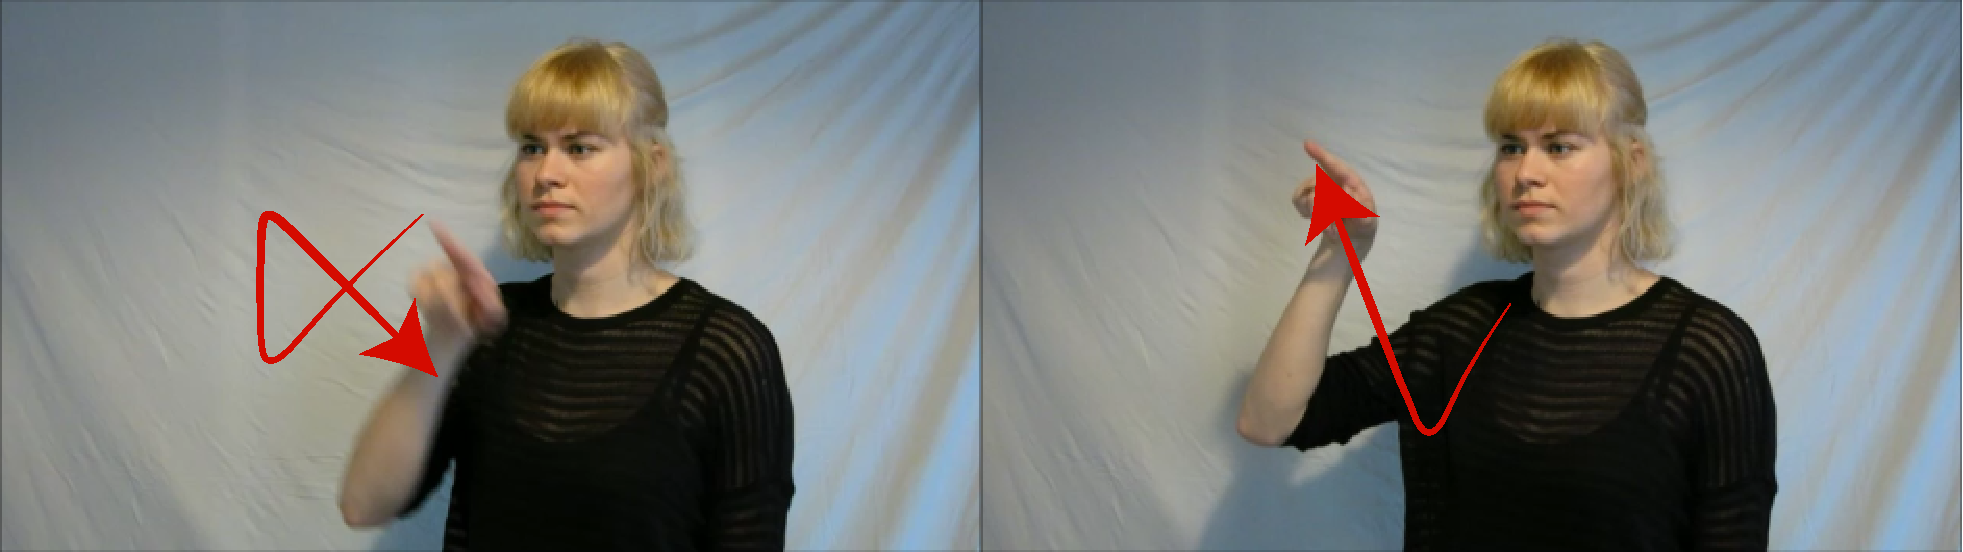
\includegraphics[resolution=300,width=0.9\textwidth]{Test1/Gestik-par/Gestik3_Pause}
	\caption{Illustration af gestik-par 3; kryds til pause og flueben til start.}
	\label{fig:GestikPar3Pause}
\end{figure}
\noindent
 %
De resterende 14 testpersoner fravælger alle GP3, illustreret på \autoref{fig:GestikPar3Pause}. De to største årsager til, at gestik-parret fravælges skyldes kompleksiteten i bevægelsen og at den simpelthen er for besværelig at udføre. I forhold til bevægelsen giver flere testpersoner udtryk for at den, foruden at være kompleks, enten er for underlig, TP3, for mærkelig, TP4, for lang og akavet, TP7 og for indviklet, TP12. I tillæg kommenterer TP17, at det bliver en større øvelse at skulle pause og starte musikken, og så vil der gå lang tid, før musikken rent faktisk bliver sat på pause. Derudover giver TP14 og TP15 udtryk for, at det ikke er sikkert, at de kan huske bevægelsen, når den skal udføres. I tillæg giver TP9 og TP14 udtryk for ikke at vil vide, hvordan musikken pauses eller startes igen. 

Af de 18 testpersoner, der har deltaget i testen, er der kun to; TP8 og TP13, som har inkluderet GP3 i deres top tre rangering. Begge testpersoner tildeler GP3 en førsteplads, lige indtil at TP8 til sidst skal gengive de fortrukne gestikker og indtil at TP13 skal lave en forbedring, hvorefter gestik-parret, i begge tilfælde, tildeles en andenplads. Årsagerne til at TP8 har inkluderet GP3 blandt de tre bedste er dels, fordi den er unik, speciel og sjov, men den gav også en fornemmelse af at det ikke bare var en knap, der blev trykket på. TP13 inkluderer derimod GP3, fordi det ikke er en typisk bevægelse at udføre og dermed vil testpersonen ikke komme til at pause musikken ved et uheld.\blankline
%
For at afgøre hvilke af de syv gestik-par, der skal fravælges, er det nødvendigt at sammenholde, hvilke gestikker testpersonerne fravælger med de gestikker, som indgår i testpersonernes top tre rangering. Der opstilles derfor en tabel over de fire fravalgte gestik-par og hvordan de indgår i testpersonernes rangering.
%
\begin{table}[H]
	\centering
	\begin{tabular}{ | p{2.4cm} | p{2.4cm} | p{2.4cm} | p{2.4cm} | p{2.4cm} |}
	\hline
		 & Gestik-par 1 & Gestik-par 2 & Gestik-par 3 & Gestik-par 4 \\ \hline
		1. Plads & 8 & 1 & 0 & 0\\ \hline
		2. Plads & 3 & 3 & 2 & 1\\ \hline
		3. Plads & 2 & 0 & 0 & 2\\ \hline
	\end{tabular}
	\caption{Oversigt over hvor ofte og hvor de fire fravalgte gestikker indgår i testpersonernes top tre rangering.}
	\label{tab:FravalgteTopTrePause}
\end{table}
\noindent
%
På baggrund af \autoref{tab:FravalgteTopTrePause} tyder det på, at det eneste gestik-par, der flerstemmigt kan ekskluderes er GP3. Dette gør sig gældende dels, fordi parret kun indgår i to testpersoners top tre og dels, fordi 14 testpersoner har fravalgt det. Derudover er GP4, illustreret på \autoref{fig:GestikPar4Pause}, kun inkluderet tre gange i testpersonernes samlede top tre rangering, jævnfør \autoref{tab:FravalgteTopTrePause}, og da gestik-parret ydermere er fravalgt, blandt andet på baggrund af det er socialt uacceptabelt, vurderes det at der ligeledes er belæg for, at ekskludere GP4 fra fremtidige undersøgelser.  
%
\begin{figure}[H]
	\centering
	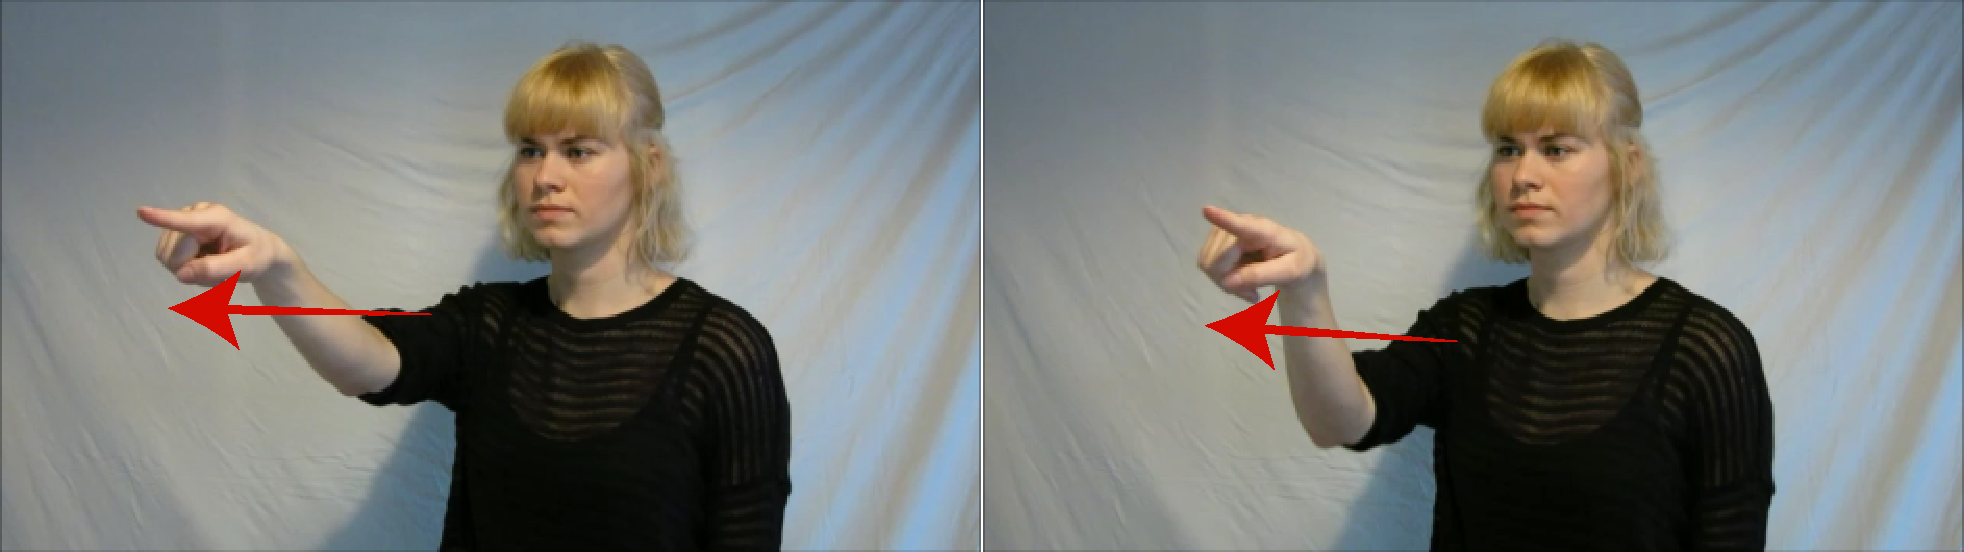
\includegraphics[resolution=300,width=0.9\textwidth]{Test1/Gestik-par/Gestik4_Pause}
	\caption{Illustration af gestik-par 4; pegefingeren peger og trykker i luften hen mod musikanlægget for henholdvis pause og start.}
	\label{fig:GestikPar4Pause}
\end{figure}
\noindent
% 
I forhold til GP2 så tyder det på, at gestik-parret kun indgår i TP3's top tre rangering, fordi testpersonen forbinder de andre forslag med mute og TP3 giver ydermere udtryk for, at det ikke giver meningen at lave et dynamisk stop-tegn, svarende til GP2. GP2 illustreres på \autoref{fig:GestikPar2Pause}. Der skal dog tages forbehold for, at TP3, ud fra testpersonens respons, virker forvirret og selvmodsigende. Ifølge TP7 bliver GP2 inkluderet i top tre rangeringen, fordi det virkede lige til og at det er det testpersonen forbinder med et stop-tegn. Årsagen til at TP10 inkluderer GP2 kan ikke direkte udledes af testpersonens udsagn, men generelt har testpersonen valgt gestikker, som var nemme at huske og med en lav risiko for, at gestikken enten gengives med en forkert bevægelse eller udføres ved et uheld. Den eneste testperson, som har tildelt GP2 en førsteplads er TP12 og årsagen til det skyldes, at testpersonen som udgangspunkt ville have valgt GP1 som den bedste og forbedret gestikken ved at tilføje bevægelsen, der gengives i GP2, jævnfør \autoref{fig:GestikPar2Pause}. Derudover giver TP12 udtryk for, at være fascineret af GP5, hvorfor det vurderes at det måske også vil tilfredsstille testpersonen, hvis GP5 blev valgt. 
%
\begin{figure}[H]
	\centering
	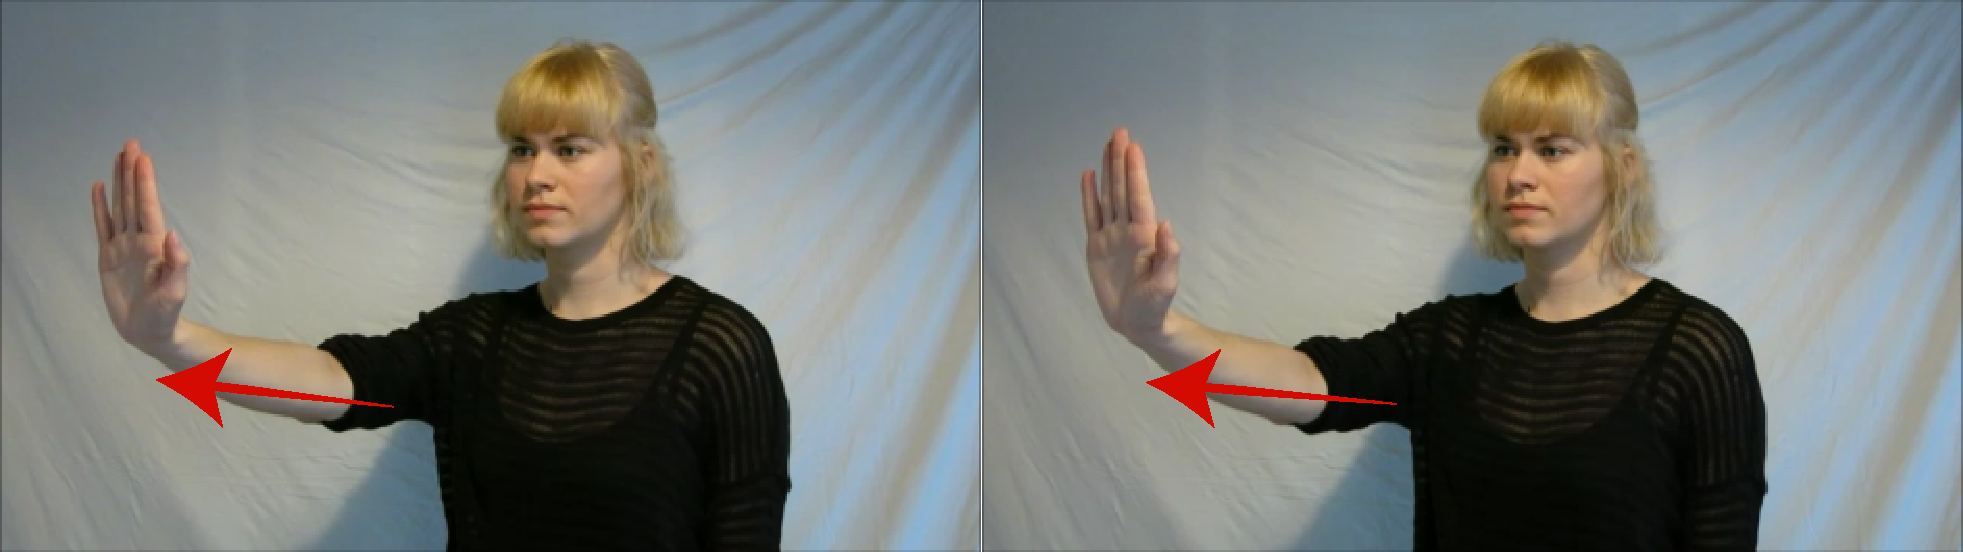
\includegraphics[resolution=300,width=0.9\textwidth]{Test1/Gestik-par/Gestik2_Pause}
	\caption{Illustration af gestik-par 2; dynamisk vertikal hånd, der starter ved brystet og ender i en udstrakt horisontal arm.}
	\label{fig:GestikPar2Pause}
\end{figure}
\noindent
% 
Argumenterne for at fravælge GP2 kan, blandt andet, sammenholdes med responsen fra både TP1 og TP8, som begge vurderer, at der er unødvendigt meget bevægelse i. Derudover blev der i \fullref{Socialaccept}, blandt andet, inddraget en undersøgelse, hvori det blev konkluderet, at testpersonerne følte sig mest komfortable, når afstanden mellem dem og selve interaktionen var lille, hvilket ligeledes understøtter argumenterne for at fravælge GP2. Selvom fokus for denne del af undersøgelsen ikke vedrører social accept, så tyder det på, at desto tættere på kroppen gestikkerne udføres, desto større er sandsynligheden for, at de indgår i testpersonernes top tre. Så baseret på de foregående argumenter og fordi GP2 kræver en bevægelse langt fra kroppen, i forhold til de andre forslag samt at gestik-parret kun fremgår fire gange i testpersonernes samlede top tre, jævnfør \autoref{tab:FravalgteTopTrePause}, så vælges det at ekskludere GP2 fra fremtidige undersøgelser. 
%
\section{Fravælgelse af gestik-par til at skifte musiknummer}
\label{app:TestresultaterSkiftDaarlig}
%
I følgende afsnit analyseres hvilke af de syv semaforiske gestik-par testpersonerne fravælger samt hvorfor testpersonerne netop fravælger disse gestik-par. På baggrund af analysen bør det være muligt at udpege hvilke semaforiske gestikker, der i hvert fald ikke skal knyttes til at skifte musiknummer. Analysen bygger på testpersonerne respons til spørgsmålet: \textit{Hvilken gestik kan du mindst lide? og hvorfor?}, hvor testpersonernes samlede data er vedlagt i \autoref{app:NoterValgAfGestikker}.
%
\begin{figure}[H]
	\centering
	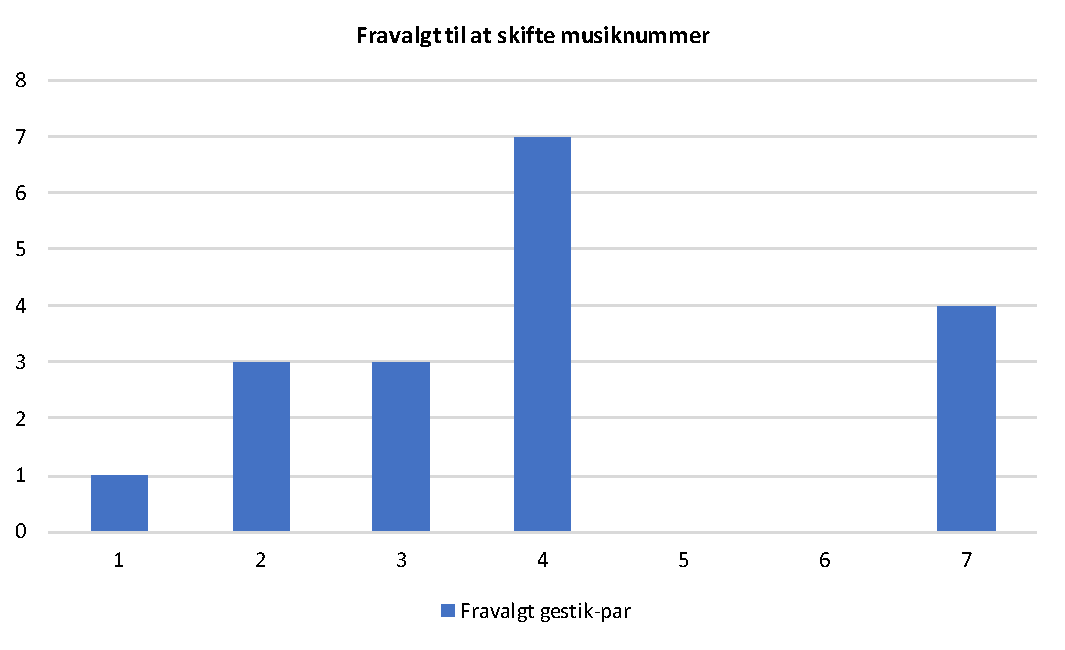
\includegraphics[resolution=300,width=0.9\textwidth]{Test1/DatabehandlingGrafer/FravalgtSkift}
	\caption{Søjlediagram over hvilke gestik-par testpersonerne fravælger i forbindelse med at skifte musiknummer frem og tilbage.}
	\label{fig:DaarligstGestikSkift}
\end{figure}
\noindent
%
På \autoref{fig:DaarligstGestikSkift} fremgår det, hvilke gestik-par de 18 testpersoner fravælger i forbindelse med at skifte musiknummer. Det fremgår tydeligt at GP4, der illustreres på \autoref{fig:GestikPar4Skift}, er det gestik-par, som flest testpersoner fravælger i forhold til de resterende gestik-par illustreret på \autoref{fig:DaarligstGestikSkift}. Derudover fravælges GP7 næstflest gange, mens GP2 og GP3 begge fravælges tre gange og GP1 fravælges en enkelt gang. Årsagen til at TP14 har valgt fravalgt GP1, begrundes med at testpersonen forestiller sig, at det er en bevægelse testpersonen vil komme til at gengive gentagende gange foran sit musikanlæg eller under en samtale. TP1, TP5 og TP16 har alle valgt GP2, som værende den de mindst kan lide, fordi gestikken er modsat af, hvad de forventer er frem og tilbage. At GP3 fravælges begrunder TP3, TP11 og TP13 med, at hvis der skulle peges i en retning, så skulle det være med pegefingeren og ikke tommelfingeren, da det er en akavet bevægelse og fordi gestikken er statisk. I den forbindelse giver TP5 udtryk for heller ikke at bryde sig om hverken GP3 eller GP7, netop fordi de er statiske.
%
\begin{figure}[H]
	\centering
	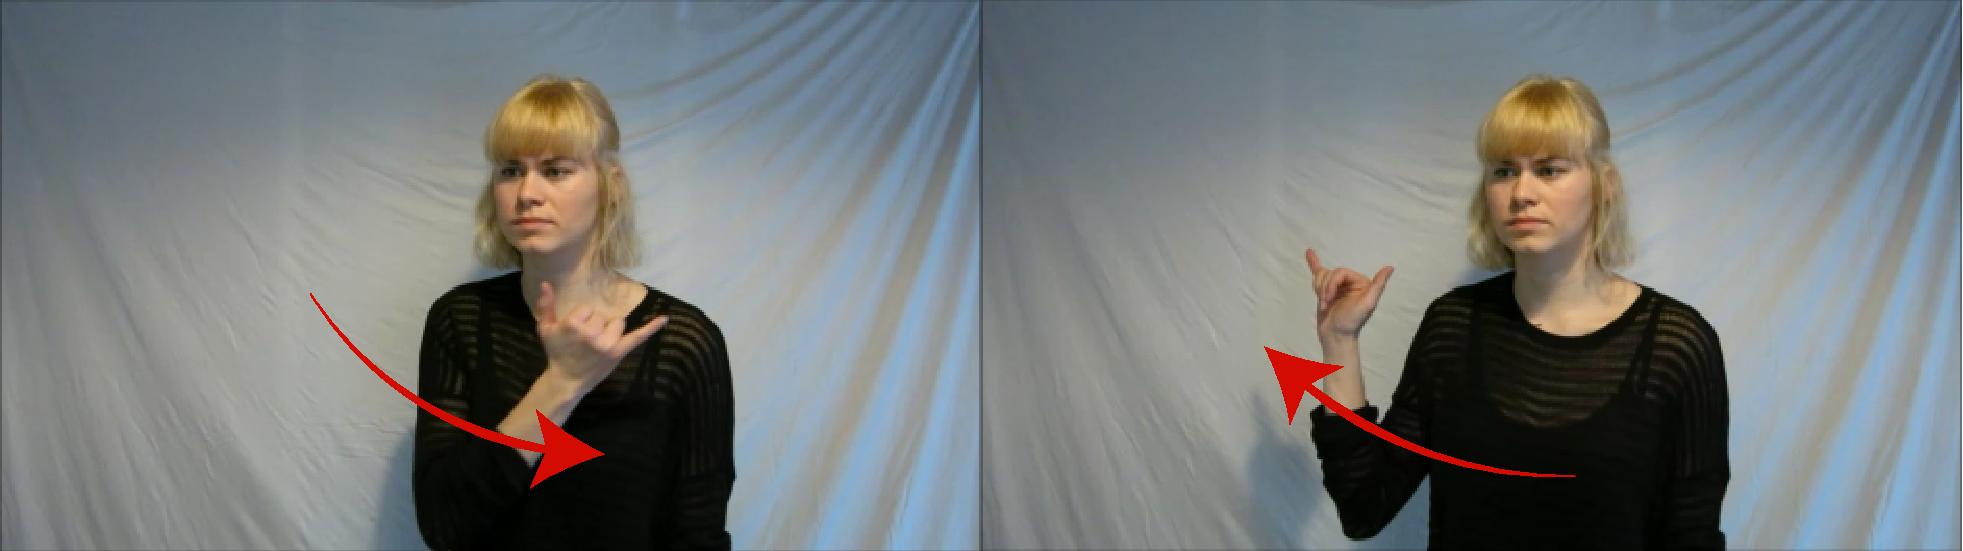
\includegraphics[resolution=300,width=0.9\textwidth]{Test1/Gestik-par/Gestik4_SkiftSang}
	\caption{Illustration af gestik-par 4; swipe fra højre mod venstre med tommel- og lillefinger strakt, mens de andre fingre bøjes for at skifte til det næste musiknummer og fra venstre mod højre for at skifte til det forrige musiknummer.}
	\label{fig:GestikPar4Skift}
\end{figure}
\noindent
%
Der er forskellige årsager til at syv testpersoner fravælger GP4. TP4 og TP6 fravælger gestikken, fordi den er mærkelig, hvor TP4 forbinder den med at skulle tage telefonen. TP8 forstår ikke, hvorfor det er lige præcis er det håndtegn, der skal bruges. TP10 oplever ikke at gestikken bringer noget nyt, men snarere at det er en besværlig version af GP5. I forhold til håndtegnet i GP4, så kommenterer TP12, at det er unaturligt at gøre noget med lillefingeren. TP7 kommenterer dels, at det er en stor armbevægelse og dels, at det er et sjovt håndtegn, som vil blive glemt, hvis det ikke bliver brugt. I tillæg kommenterer TP18 ligeledes, at det er en unaturlig gestik, som vil blive glemt. Dog pointerer testpersonen, at det er en effektiv gestik i og med at den ikke vil blive lavet ved en fejl.
%
\begin{figure}[H]
	\centering
	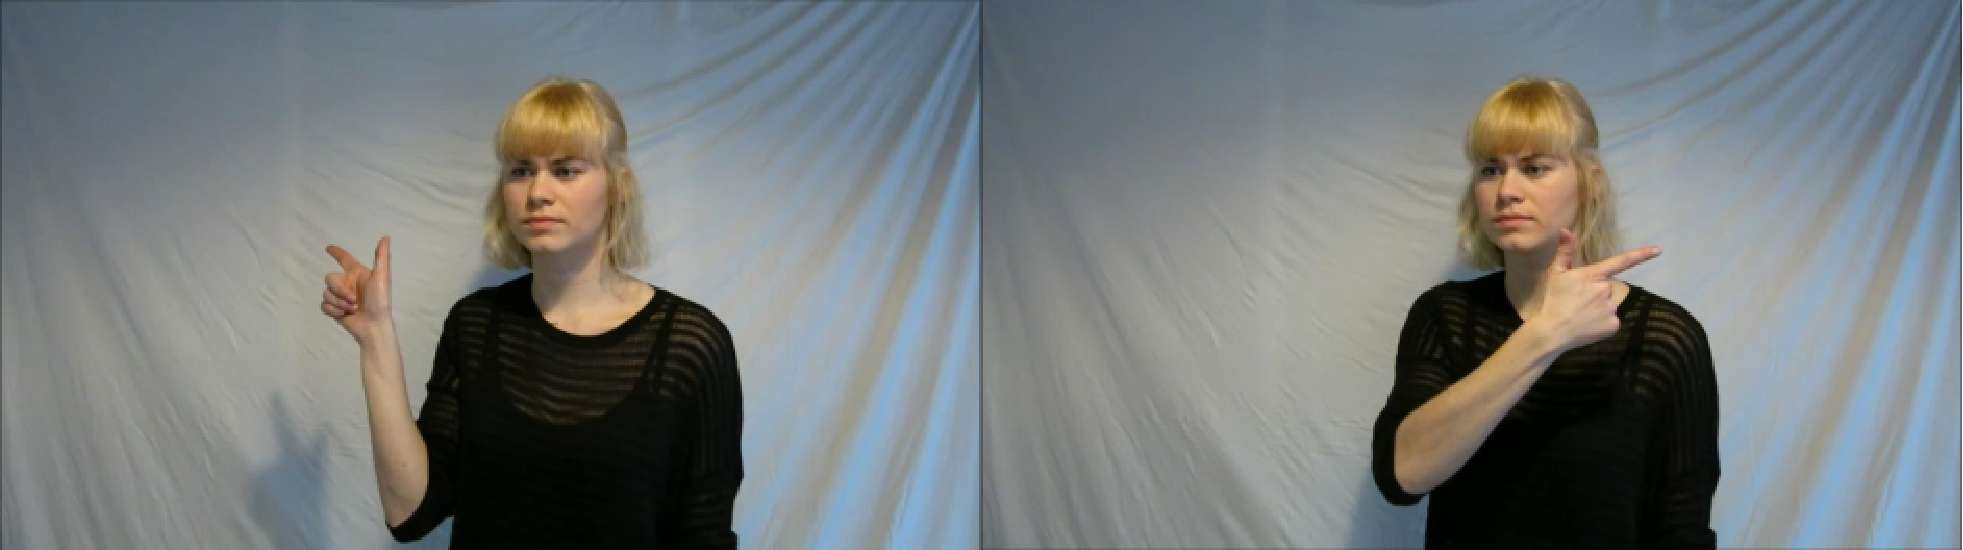
\includegraphics[resolution=300,width=0.9\textwidth]{Test1/Gestik-par/Gestik7_SkiftSang}
	\caption{Illustration af gestik-par 7; peg med tommel- og pegefinger strakt i den retning musiknummeret skal skifte i. Først frem og derefter til det forrige musiknummer.}
	\label{fig:GestikPar7Skift}
\end{figure}
\noindent
% 
Årsagen til at GP7 fravælges skyldes ifølge TP2, TP9 og TP17 dels, at den virkede mærkelig, dels, at den ikke blev opfattet og dels, at den minder om en pistol. GP7 illustreres på \autoref{fig:GestikPar7Skift}. Ligesom GP3 blandt andet blev fravalgt, fordi den er statisk, så fravælger TP15 af samme årsag GP7.\blankline
%
For at afgøre hvilke af de syv gestik-par, der skal fravælges, er det nødvendigt at sammenholde, hvilke gestikker testpersonerne fravælger med de gestikker, som indgår i testpersonernes top tre rangering. Der opstilles derfor en tabel over de fem fravalgte gestik-par og hvordan de indgår i testpersonernes rangering.    
%
\begin{table}[H]
	\centering
	\begin{tabular}{ | p{1.5cm} | p{2.1cm} | p{2.1cm} | p{2.1cm} | p{2.1cm} | p{2.1cm} |}
	\hline
		 & Gestik-par 1 & Gestik-par 2 & Gestik-par 3 & Gestik-par 4 & Gestik-par 7 \\ \hline
		1. Plads & 10 & 3 & 1 & 0 & 0\\ \hline
		2. Plads & 2 & 3 & 3 & 0 & 1\\ \hline
		3. Plads & 0 & 0 & 7 & 5 & 2\\ \hline
	\end{tabular}
	\caption{Oversigt over hvor ofte og hvor de fem fravalgte gestikker indgår i testpersonernes top tre rangering.}
	\label{tab:FravalgteTopTreSkift}
\end{table}
\noindent
%
På baggrund af \autoref{tab:FravalgteTopTreSkift} sammenholdt med \autoref{fig:DaarligstGestikSkift}, tyder det på, at GP4 og GP7 kan ekskluderes fra fremtidige undersøgelser. Det skyldes at selvom GP4 indgår fem gange i testpersonernes top tre, så fravælges gestik-parret af syv testpersoner. Derudover tyder det på, at de fem testpersoner, som har inkluderet GP4 i deres top tre, har gjort det på baggrund af bevægelsen snarre end kombinationen af både håndtegnet og bevægelsen. GP7 ekskluderes, da gestik-parret kun indgår tre gange i testpersonernes samlede top tre og da den derudover fravælges af fire testpersoner. 
%
\begin{figure}[H]
	\centering
	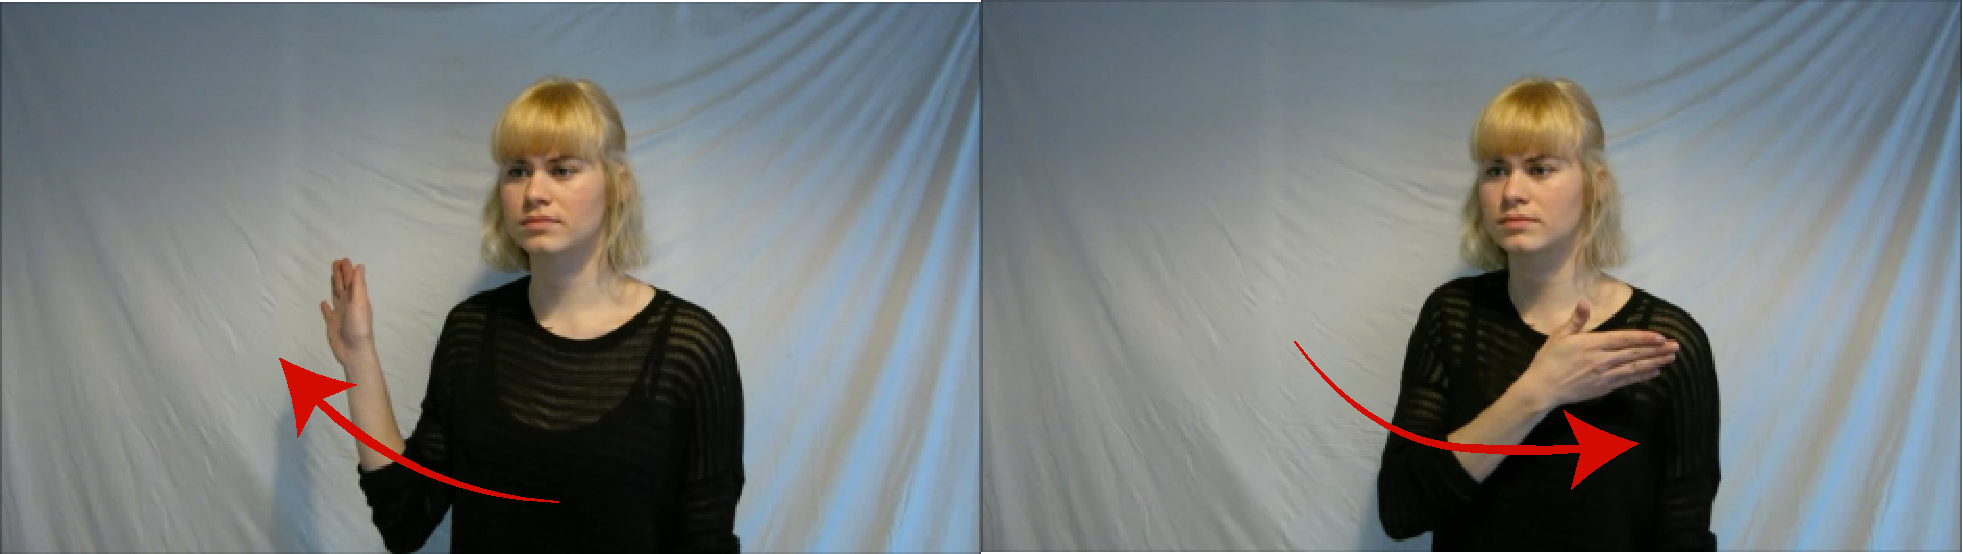
\includegraphics[resolution=300,width=0.9\textwidth]{Test1/Gestik-par/Gestik2_SkiftSang}
	\caption{Illustration af gestik-par 2; swipe-bevægelse fra venstre mod højre for at skifte til det næste musiknummer og fra højre mod venstre for at skifte til det forrige musiknummer.}
	\label{fig:GestikPar2Skift}
\end{figure}
\noindent
%
De tre testpersoner, som fravælger GP2, gør det formentligt, fordi de har en mental model af, at hvis der swipes fra højre mod venstre så afspilles det næste musiknummer i playlisten, modsat hvis der swipes fra venstre mod højre så afspilles det forrige musiknummer. GP2 illustreres på \autoref{fig:GestikPar2Skift}. De tre testpersoner, der har tildelt GP2 en førsteplads, har formentligt den modsatte mentale model af, hvilken swipe-bevægelse, der skal udføres for at skifte til det næste musiknummer. For at det kan afgøres, hvorvidt GP2 skal ekskluderes eller ej, så er det nødvendigt at undersøge nærmere, hvilke gestik-par de seks testpersoner, som har inkluderet GP2 i deres top tre, ellers har inkluderet. 
%
\begin{table}[H]
	\centering
	\begin{tabular}{ | p{3cm} | p{3cm} | p{3cm} | p{3cm} |}
	\hline
		 & 1. Plads & 2. Plads & 3. Plads \\ \hline
		Testperson 4 & Gestik-par 2 & Gestik-par 5 & Gestik-par 3 \\ \hline
		Testperson 17 & Gestik-par 2 & Gestik-par 3 & Gestik-par 4 \\ \hline
		Testperson 18 & Gestik-par 2 & Gestik-par 1 & Gestik-par 3 \\ \hline
		Testperson 8 & Gestik-par 3 & Gestik-par 2 & Gestik-par 7 \\ \hline
		Testperson 12 & Gestik-par 1 & Gestik-par 2 & Gestik-par 5\\ \hline
		Testperson 15 & Gestik-par 1 & Gestik-par 2 & Gestik-par 5 \\ \hline
	\end{tabular}
	\caption{Oversigt over de seks testpersoner, som enten har tildelt GP2 en første eller en andenplads i top tre, samt hvilke gestik-par de ellers har inkluderet.}
	\label{tab:GestikPar2ITopTre}
\end{table}
\noindent
%
Sammenholdes TP4's top tre rangering med testpersonens udsagn og bevægelser i videooptagelserne, så tyder det på, at denne testperson har en mental model af, at hvis der swipes fra højre mod venstre så afspilles det forrige musiknummer kontra et swipe fra venstre mod højre, som vil afspille det næste musiknummer. I \autoref{app:VideooptagelseValgAfGestikkerTestpersoner} forefindes videomateriale for den pågældende situation. Testpersonen kommenterer ydermere, at GP5 også vil fungere, såfremt retning var omvendt, svarende til hvad der gengives i GP2, som illustreres på \autoref{fig:GestikPar2Skift}. TP17, som ligeledes har tildelt gestik-par 2 en førsteplads, udfører også de korrekte bevægelser i forhold til testpersonens egne kommentarer. Dog opstår der usikkerhed, når testpersonen afslutningsvist skal gengive sine fortrukne gestikker. Efter en diskusion med testlederen konkluderer TP17 dog at det stadig er GP2, der er bedst. Selvom TP18 virker sikker i sit valg om, at det er GP2, der er det bedste gestik-par, så gengiver testpersonen rent faktisk bevægelserne fra gestik-par 1, dog med venstre hånd, hvilket forefindes i videomaterialet vedlagt i \autoref{app:VideooptagelseValgAfGestikkerTestpersoner}. Når testpersonen i tillæg forklarer, hvad swipe-bevægelserne gør i forhold til at skifte til det forrige eller det næste musiknummer, relaterer det sig ligeledes til GP1. Det er derfor ikke til at vide, hvorfor testpersonen har rangeret GP2 højere end GP1. Det tyder derfor på at den eneste testperson, der med sikkerhed vil vælge swipe-bevægelserne i GP2 som en førsteprioritet, er TP4. 

Rettes fokus mod de tre testpersoner, som har rangeret GP2 på en andenplads, så tyder det på at de to testpersoner, som har tildelt GP1 en førsteplads, hovedsageligt har inkluderet GP2 på grund af bevægelsen. Dog kommenterer TP15, at GP2 er modsat af hvad testpersonen finder logisk. TP12 pointerer, at det var svært at adskille GP1 fra GP2. TP8 har derimod rangeret GP2 mellem de to statiske gestik-par og når testpersonen gengiver bevægelserne i GP2, stemmer det både overens med testpersons udsagn samt hvordan gestik-parret er designet. Det tyder derfor på at testpersonen rent faktisk har valgt GP2, fordi det stemmer overens med testpersonens mentale model.\blankline 
%
Ud af de seks testpersoner er det kun TP4 og TP8, der giver entydigt udtryk for, at deres mentale model af GP2 stemmer overens både med deres bevægelser og deres udsagn. Derudover er der i Bang $\&$ Olufsens produkter desuden truffet en designbeslutning om, at en swipe-bevægelse fra højre mod venstre resulterer i at det er det næste musiknummer afspilles, da dette stemmer overens med at trække det næste musiknummer frem. På baggrund af den foregående analyse og da det ikke ønskes at gå i mod Bang $\&$ Olufsens designvalg, vurderes det derfor, at der er tilstrækkeligt belæg for at ekskludere GP2. 

På baggrund af foregående analyse forefindes der ikke et tilstrækkeligt belæg for hverken at ekskludere GP1 eller GP3, hvorfor disse vil undersøges nærmere. \blankline
%
GP6 er ikke fravalgt nogle gange, men er kun tildelt en første plads én gang; af TP13, jævnfør \autoref{tab:GestikParITopTreSkift}. GP6 illustreres på \autoref{fig:GestikPar6Skift}. Testpersonen formår ikke at præcisere, hvorfor GP6 rangeres højere end GP5, men testpersonen giver udtryk for bedst at kunne lide de gestikker, hvor hånden bevæges på en bestemt måde samt de gestikker, som indeholder et specielt håndtegn. I de to tilfælde, hvor GP6 indgår på en anden plads, så er det efter GP5, hvor det ud fra testpersonernes udsagn vurderes, at det skyldes dels håndtegnet og dels bevægelsen. Når GP6 indgår på en tredje plads så har testpersonerne i begge tilfælde tildelt GP1 en førsteplads og enten GP5 eller GP3 en andenplads. 
%
\begin{figure}[H]
	\centering
	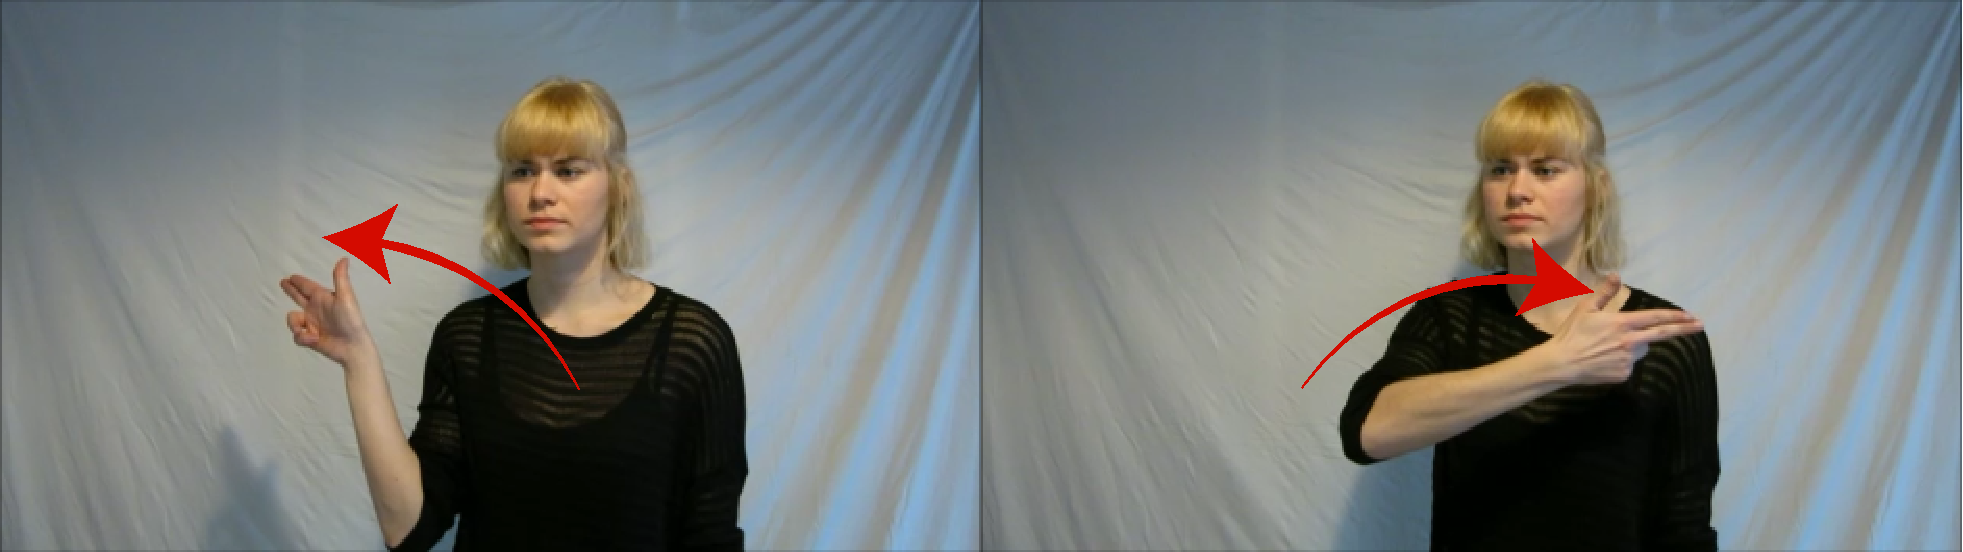
\includegraphics[resolution=300,width=0.9\textwidth]{Test1/Gestik-par/Gestik6_SkiftSang}
	\caption{Illustration af gestik-par 6; bue med pege- og langefinger fra venstre mod højre for at skifte til det næste musiknummer og fra højre mod venstre for at skifte til det forrige musiknummer.}
	\label{fig:GestikPar6Skift}
\end{figure}
\noindent
%                
Der er kun én testperson, som har tildelt GP6 en førsteplads og derudover vurderes det, at når GP6 indgår enten på en anden- eller tredjeplads, så er testpersonernes ønsker dækket af et eller flere af de gestik-par, som de har rangeret over. Det vurderes derfor at der er belæg for at ekskludere GP6.
%
\section{Fravælgelse af gestik-par til at skrue op og ned for musikken}
\label{app:TestresultaterVolumenDaarlig}
%
I følgende afsnit analyseres hvilke af de ni semaforiske gestik-par testpersonerne fravælger samt hvorfor testpersonerne netop fravælger disse gestik-par. På baggrund af analysen bør det være muligt at udpege hvilke semaforiske gestikker, der i hvert fald ikke skal knyttes til at skrue op og ned for musikken. Analysen bygger på testpersonerne respons til spørgsmålet: \textit{Hvilken gestik kan du mindst lide? og hvorfor?}, hvor testpersonernes samlede data er vedlagt i \autoref{app:NoterValgAfGestikker}.
%
\begin{figure}[H]
	\centering
	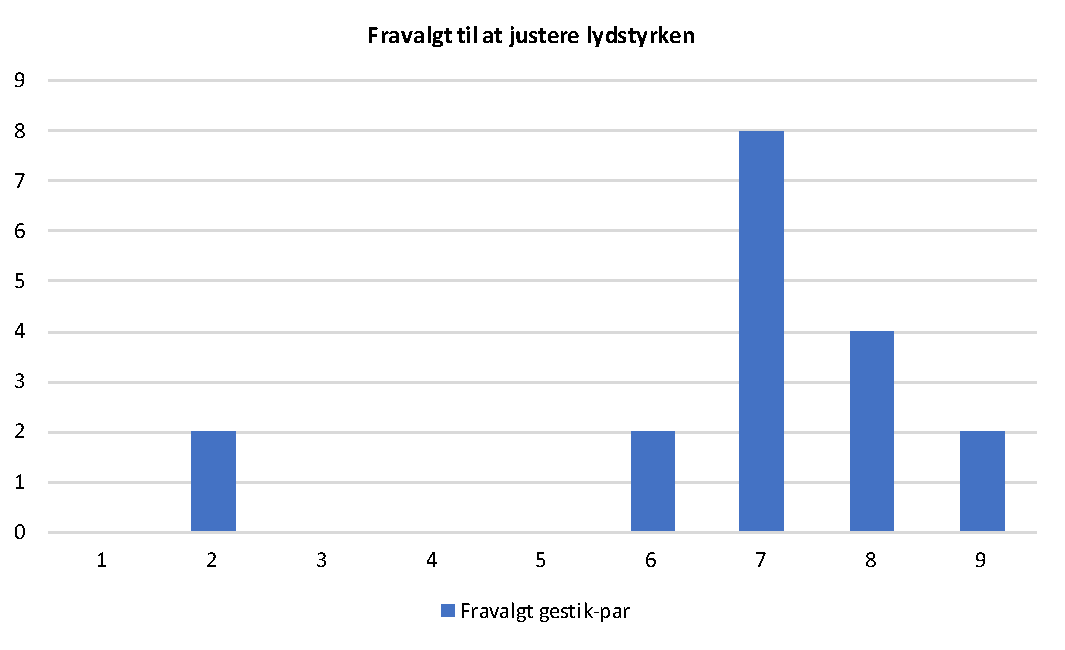
\includegraphics[resolution=300,width=0.9\textwidth]{Test1/DatabehandlingGrafer/FravalgtVolumen}
	\caption{Søjlediagram over hvilke gestik-par testpersonerne fravælger i forbindelse med at skrue op og ned for musikken.}
	\label{fig:DaarligstGestikVolumen}
\end{figure}
\noindent
%
På \autoref{fig:DaarligstGestikVolumen} fremgår det, hvilke gestik-par de 18 testpersoner fravælger i forbindelse med at skrue op og ned for musikken. Det fremgår tydeligt, at testpersonerne hyppigst fravælger GP7, da gestik-parret i alt er fravalgt otte gange, og ikke indgår på en eneste top tre rangering, jævnfør \autoref{tab:GestikParITopTreVolumen}. GP7 illustreres på \autoref{fig:GestikPar7Volumen}. Årsagen til at GP7 fravælges varierer mellem de otte testpersonerne, som har valgt gestik-parret. TP2 har svært ved at vurdere, hvilken vej der er op og hvilken vej, der er ned. Ifølge TP3 er GP7 underlig og derudover så giver det ikke mening. At gestik-parret ikke giver mening pointere TP15 også og tilføjer, at det er en mellemting mellem GP5 og GP6. TP4 fravælger gestikken, fordi den er mærkelig, hvilket også er en af årsagerne til at TP11 fravælger gestik-parret. Derudover kommenterer TP11, at det kræver koncentration at gengive en bue, hvilket er en del af bevægelsen. Da formålet med at anvende semaforiske gestikker til at interagere med Bang $\&$ Olufsen's fremtidige musikanlæg, blandt andet er for at interaktionen på sigt kan foregå i den perifere opmærksomhed, så er det ikke hensigtsmæssigt at gestikkerne kræver mere koncentration end andre løsninger. Derudover påpeger TP10, at GP7 er væsentligt mindre intuitiv end de andre forslag og dertil er det svært at vurdere den nødvendige bevægelsesmængde for at skrue op og ned. Ifølge TP6 så er GP7 det par, som skiller sig mest ud i forhold til de andre forslag, hvilket er årsagen til at parret fravælges. TP14's respons afviger fra de andre testpersoners, i det at TP14 fravælger GP7, fordi testpersonen anser det som værende en meget naturlig bevægelse, som testpersonen giver udtryk for at vil komme til at lave ubevidst.
%
\begin{figure}[H]
	\centering
	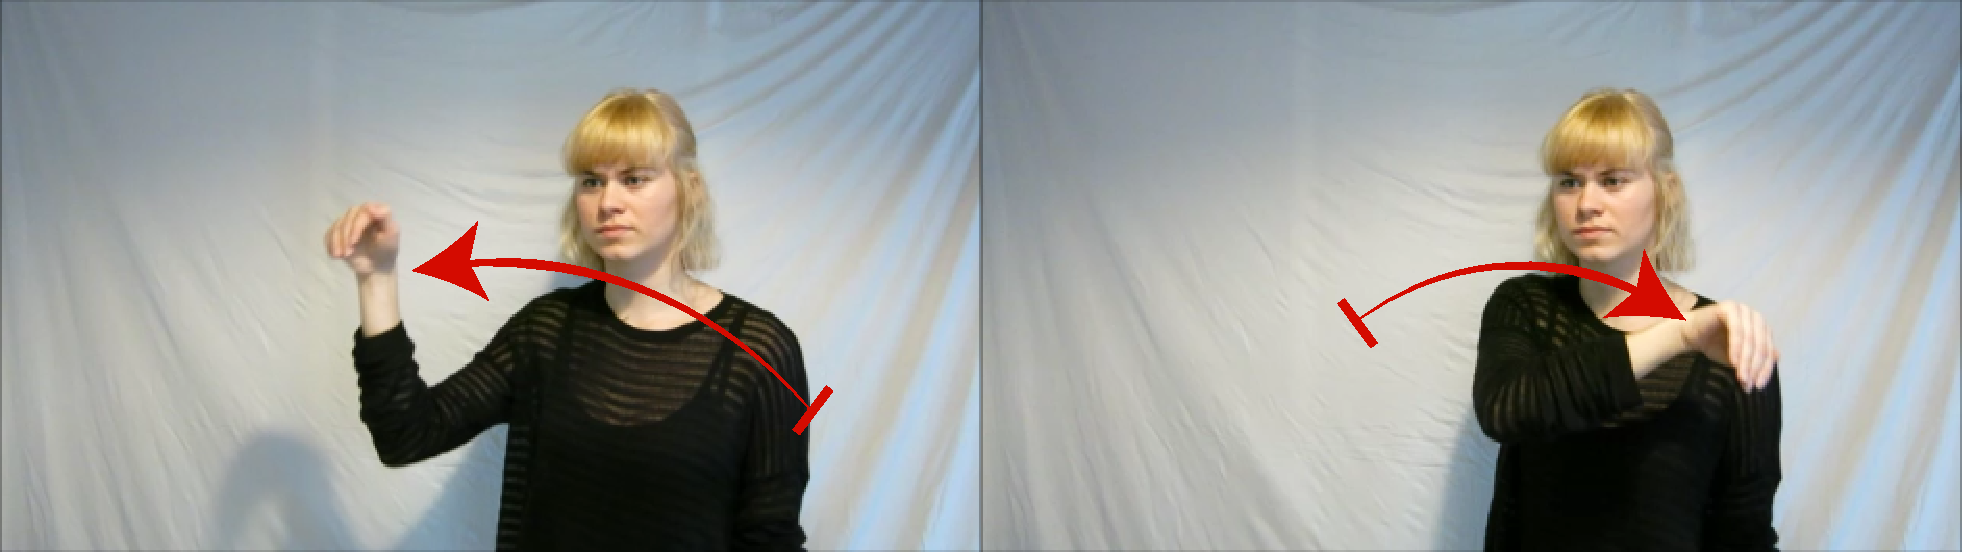
\includegraphics[resolution=300,width=0.9\textwidth]{Test1/Gestik-par/Gestik7_Volumen}
	\caption{Illustration af gestik-par 7; krum hånd bevæges i en bue fra venstre mod højre for at skrue op og fra højre mod venstre for at skrue ned, svarende til hvordan det gøres på A9, \parencite{WEB:BeoplayA9}.}
	\label{fig:GestikPar7Volumen}
\end{figure}
\noindent
%
Selvom GP7 blev inkluderet som et forsøg på at overføre gestikken, der anvendes til at skrue op og ned på en A9, \parencite{WEB:BeoplayA9}, til en semaforisk gestik, så er GP7 det par, som oftes fravælges og som ikke indgår i nogen af testpersonernes top tre, hvorfor gestik-parret ekskluderes.
%
\begin{figure}[H]
	\centering
	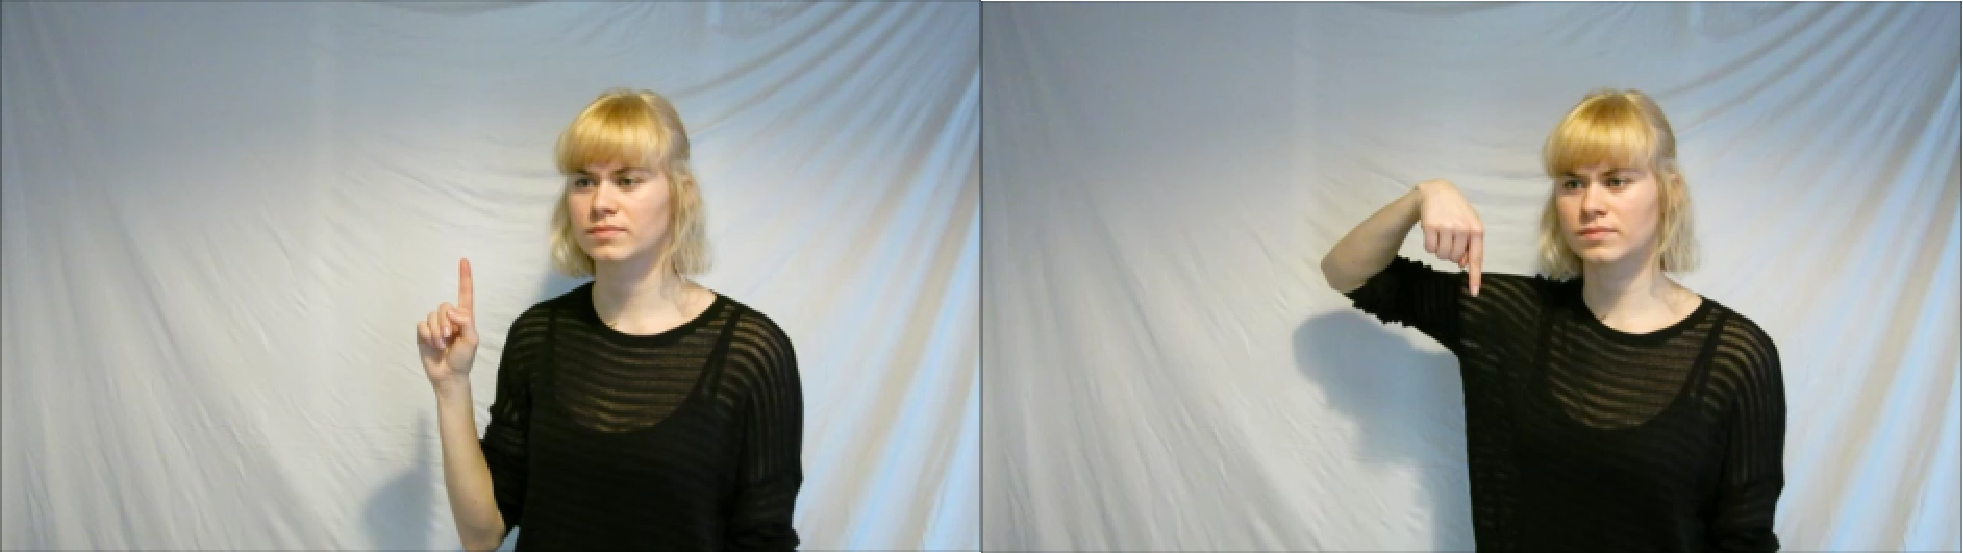
\includegraphics[resolution=300,width=0.9\textwidth]{Test1/Gestik-par/Gestik8_Volumen}
	\caption{Illustration af gestik-par 8; pegefingeren peger op for at skrue op og peger ned for at skrue ned.}
	\label{fig:GestikPar8Volumen}
\end{figure}
\noindent
%
To ud af de fire testpersoner, som fravælger GP8, illustreret på \autoref{fig:GestikPar8Volumen}, giver udtryk for at det er besværligt at pege nedad. Den ene af de to, TP18, giver stærkt udtryk for, at det er både besværligt og ubehagligt at pege nedad samt at have sin arm i den position. Den anden af de to testpersoner, TP9, giver udtryk for, at det besværligt at gengive og det er underligt at pege nedad. Derudover pointerer TP9, at det er svært at kontrollere, hvor meget der enten skal skrues og eller ned, hvilket også er årsagen til at TP5 fravælger GP8. Den sidste af de fire testpersoner, TP13, fravælger GP8, fordi der mangler bevægelse og fordi det er noget testpersonen godt kunne forestille sig komme til at gøre ved et uheld. \blankline 
%
Der er to forskellige årsager til, hvorfor GP2 fravælges af TP12 og TP16. TP12 fravælger GP2, fordi testpersonen ikke bryder sig om cirkelbevægelsen, selvom testpersonen pointerer, at det burde virke naturligt og det egentlig er sådan der normaltvist skrues op på et musikanlæg. Det skal dog pointeres at TP12 ikke endegyldigt fastslår, at det er GP2, der er værst, da testpersonen egentlig heller ikke bryder sig om GP1. Grunden til at det fremgår, at TP12 har valgt GP2 som værende dårligst, er på baggrund af de bevægelser, der opstår når testpersonen skal forklare hvorfor der vælges som der gør. I dette tilfælde stemte bevægelsen overens med bevægelsen i GP2. Årsagen til at GP2 fravælges af TP16 er, fordi bevægelsen er modsat af hvad testpersonen forventer. Det skal dog pointeres, at der ved GP2 skrues op for musikken ved at dreje hånden med uret og skrues ned ved at dreje hånden mod uret, hvilket er det testpersonen egentlig forventer. Det tyder derfor på at TP16 har misforstået videooptagelsen af GP2. Testlederen spørger derfor ind til hvordan GP2 kunne gøres bedre, hvor TP16 først og fremmest foreslår, at bevægelsen foregår i den rigtige retning og derudover foreslår testpersonen, at gestikken skulle være mere ligesom GP1, hvor testpersonen referer til armens position. 

GP6 fravælges af TP9, fordi det vil være svært, at gengive bevægelsen med et barn på armen, hvilket også gør sig gældende for GP5. GP6 illustreres på \autoref{fig:GestikPar6Volumen}. TP17 fravælger GP6 fordi det er ulogisk at lave den bevægelse i forbindelse med musik og derudover virker det mærkeligt at begge hænder skal være involveret. 

Ifølge TP7 så fravælges GP9, fordi den ikke tillader kontrol over hvor meget der skrues op og ned, hvorimod TP8 fravælger GP9 fordi testpersonen vil have det akavet med at lave den bevægelse.\blankline
%
For at afgøre hvilke af de ni gestik-par, foruden GP7, som allerede er ekskluderet, der skal fravælges, er det nødvendigt at sammenholde, hvilke gestikker testpersonerne fravælger med de gestikker, som indgår i testpersonernes top tre rangering. Der opstilles derfor en tabel over de fem fravalgte gestik-par og hvordan de indgår i testpersonernes rangering.    
%
\begin{table}[H]
	\centering
	\begin{tabular}{ | p{1.5cm} | p{2.1cm} | p{2.1cm} | p{2.1cm} | p{2.1cm} | p{2.1cm} |}
	\hline
		 & Gestik-par 2 & Gestik-par 6 & Gestik-par 7 & Gestik-par 8 & Gestik-par 9 \\ \hline
		1. Plads & 4 & 1 & 0 & 0 & 2\\ \hline
		2. Plads & 2 & 2 & 0 & 0 & 1\\ \hline
		3. Plads & 3 & 1 & 0 & 2 & 3\\ \hline
	\end{tabular}
	\caption{Oversigt over hvor ofte og hvor de fem fravalgte gestikker indgår i testpersonernes top tre rangering.}
	\label{tab:FravalgteTopTreVolumen}
\end{table}
\noindent
%
På baggrund af \autoref{tab:FravalgteTopTreVolumen} hvor GP9 fremgår seks gange i testpersonernes top tre rangering sammenholdt med \autoref{fig:DaarligstGestikVolumen} samt testpersonernes begrundelser for, hvorfor de fravælger GP9, vurderes det, at der er ikke er belæg for at ekskludere GP9. Det vurderes ydermere, at der ikke forefindes tilstrækkeligt belæg for at ekskludere GP2, for selvom det ikke kan antages med sikkerhed, at TP16 ville have udpeget et andet gestik-par, i tilfælde af at testpersonen ikke havde misforstået bevægelsesretningen, så tyder det på, at det godt kunne være tilfældet. I så fald er det kun TP12, som har givet udtryk for at en cirkulærbevægelse ikke foretrækkes. Da det heller ikke entydigt kan konkluderes, hvorvidt TP12 mindst kan lide GP2 i forhold til GP1 og da GP2 sammenlagt indgår ni gange i testpersonernes top tre, jævnfør \autoref{tab:FravalgteTopTreVolumen}, vurderes det at der ikke er belæg for at ekskludere GP2 .
%
Baseret på \autoref{tab:FravalgteTopTreVolumen} hvor GP8 kun indgår to gange i testpersonernes samlede top tre rangering sammenholdt med \autoref{fig:DaarligstGestikVolumen} samt testpersonernes begrundelser for, hvorfor de fravælger GP8, vurderes det at der er belæg for at ekskludere GP8. 
%
\begin{figure}[H]
	\centering
	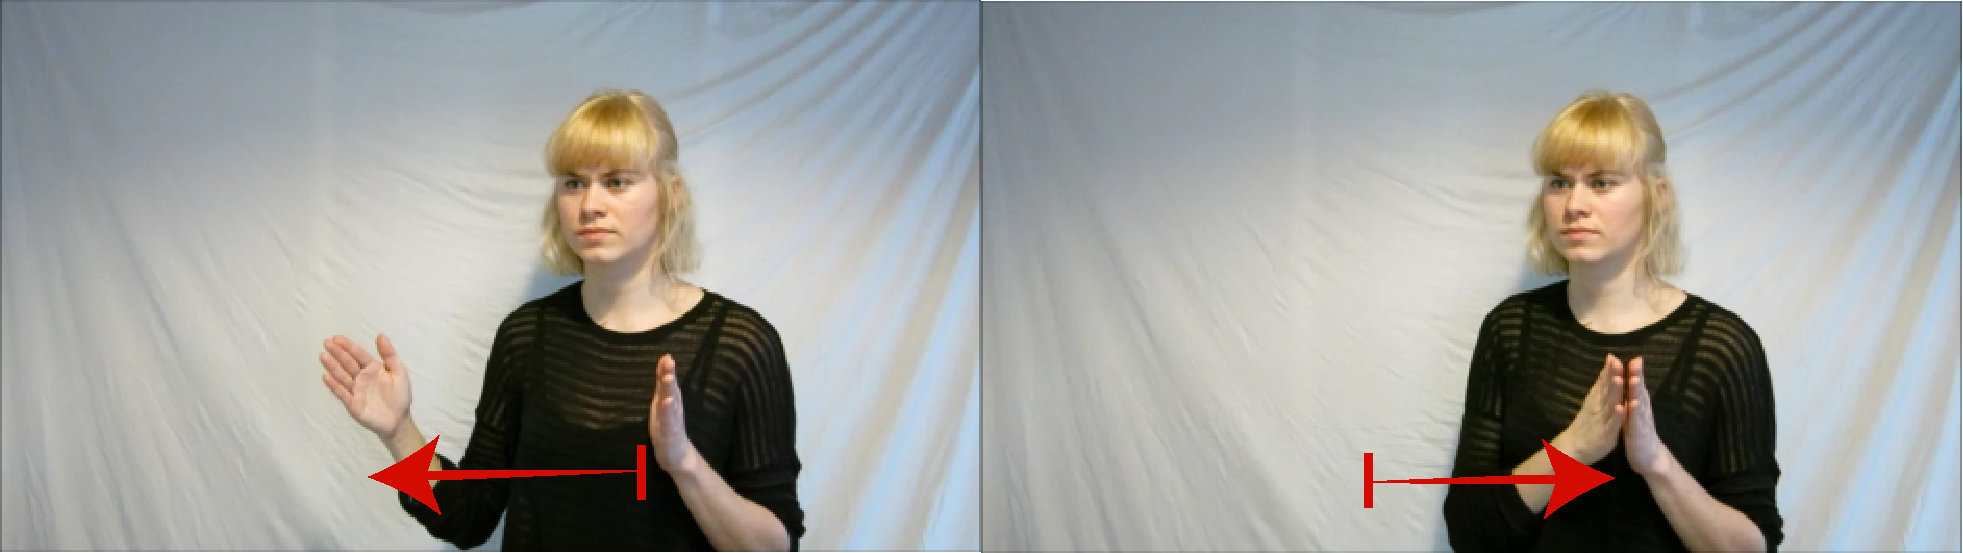
\includegraphics[resolution=300,width=0.9\textwidth]{Test1/Gestik-par/Gestik6_Volumen}
	\caption{Illustration af gestik-par 6; vertikal ikke-dominant hånd holdes stationær, ems den dominante hånd ligeledes holdes vertikal og bevægelser sig væk fra den ikke-dominante hånd i en horisontal bevægelse for at skrue op og for at skrue ned bevæges den dominante hånd mod den ikke-dominante hånd.}
	\label{fig:GestikPar6Volumen}
\end{figure}
\noindent
% 
For at have belæg for at ekskludere GP6, er det nødvendigt at inkludere hvad testpersonerne, som har rangeret GP6 i deres top tre, har kommenteret. Ifølge TP1 så indgår GP6 på en andenplads dels, fordi den følger et princip om noget, der er større eller mindre, jævnfør \autoref{fig:GestikPar6Volumen}, og dels, fordi bevægelsen er naturlig. Det tyder på, at TP14 rangerer gestikkerne alt efter hvad der føles akavet og unaturligt i frygt for at komme til at lave gestikkerne ved et uheld, hvilket er årsagen til at TP14 har tildelt GP6 en andenplads. TP2 forklarer, at årsagen til at GP6 rangeres på en tredjeplads er, fordi den minder om GP4 og GP5 bare sidelæns, men at det ikke giver lige så meget mening, som de to andre. Baseret på TP5's udsagn tyder det på, at årsagen til at GP6 tildeles en førsteplads er, fordi testpersonen ønsker at have fuld kontrol over, hvor meget der skrues op og ned, hvilket testpersonen oplever ved at bruge begge hænder, jævnfør \autoref{fig:GestikPar6Volumen}. Grunden til at testpersonen vælger GP6 fremfor GP5 skyldes, at GP6 fylder mindre i rummet. Sammenholdes de fire testpersoners udsagn med, hvordan de rent faktisk gengiver GP6, så tyder det på, at ingen af testpersonerne formår, at gengive bevægelsen korrekt. Det fremgår af optagelserne, at ingen af de fire testpersoner formår at fastholde deres ikke-dominante hånd som reference og derfra kontrollere, hvor meget der skal skrues op eller ned med den dominante hånd. Til gengæld tyder det på, at de fire testpersoner fortolker og gengiver GP6 ens; begge hænder bevæger sig horisontalt mod eller væk fra hinanden med håndfladerne vendt ind mod hinanden. 

Så med udgangspunkt i testpersonerne begrundelser for, hvorfor de enten fravælger GP6 eller inkluderer GP6 i deres top tre, samt hvad de rent faktisk gør, når de gengiver gestik-parret, så vurderes det, at der er belæg for at ekskludere GP6.  





